%----------------------------------------------------------------------------------------
%   PACKAGES AND THEMES
%----------------------------------------------------------------------------------------

\documentclass[aspectratio=169]{beamer}

\mode<presentation> {

% The Beamer class comes with a number of default slide themes
% which change the colors and layouts of slides. Below this is a list
% of all the themes, uncomment each in turn to see what they look like.

%\usetheme{default}
%\usetheme{AnnArbor}
%\usetheme{Antibes}
%\usetheme{Bergen}
%\usetheme{Berkeley}
%\usetheme{Berlin}
%\usetheme{Boadilla}
%\usetheme{CambridgeUS}
%\usetheme{Copenhagen}
%\usetheme{Darmstadt}
%%%%%%%\usetheme{Dresden}
%\usetheme{Frankfurt}
%\usetheme{Goettingen}
%\usetheme{Hannover}
%\usetheme{Ilmenau}
%\usetheme{JuanLesPins}
\usetheme{Luebeck}
%\usetheme{Madrid} 
%\usetheme{Malmoe}
%\usetheme{Marburg}
%\usetheme{Montpellier}
%\usetheme{PaloAlto}
%\usetheme{Pittsburgh}
%\usetheme{Rochester}
%\usetheme{Singapore}
%\usetheme{Szeged}
%\usetheme{Warsaw}

% As well as themes, the Beamer class has a number of color themes
% for any slide theme. Uncomment each of these in turn to see how it
% changes the colors of your current slide theme.

%\usecolortheme{albatross}
%%%%%\usecolortheme{beaver}
%\usecolortheme{beetle}
%\usecolortheme{crane}
%\usecolortheme{dolphin}
%\usecolortheme{dove}
%\usecolortheme{fly}
%\usecolortheme{lily}
%\usecolortheme{orchid}
%\usecolortheme{rose}
%\usecolortheme{seagull}
%\usecolortheme{seahorse}
%\usecolortheme{whale}
%\usecolortheme{wolverine}
\usecolortheme{default}

%\setbeamertemplate{footline} % To remove the footer line in all slides uncomment this line
%\setbeamertemplate{footline}[page number] % To replace the footer line in all slides with a simple slide count uncomment this line

%\setbeamertemplate{navigation symbols}{} % To remove the navigation symbols from the bottom of all slides uncomment this line
}


\addtobeamertemplate{navigation symbols}{}{%
    \usebeamerfont{footline}%
    \usebeamercolor[fg]{footline}%
    \hspace{1em}%
    \insertframenumber/\inserttotalframenumber
}



\usepackage{graphicx} % Allows including images
\usepackage{booktabs} % Allows the use of \toprule, \midrule and \bottomrule in tables
\usepackage[utf8]{inputenc}

\usepackage{ragged2e}
\usepackage{lmodern}
\usepackage{array}
\usepackage[normalem]{ulem}
\usepackage{microtype}

\usepackage{graphicx}
\graphicspath{ {images/} }

\setbeamerfont{footnote}{size=\tiny}

\renewcommand{\figurename}{Figura}

%----------------------------------------------------------------------------------------
%   TITLE PAGE
%----------------------------------------------------------------------------------------


\title[Projeto de Visualização]{Técnica de Visualização Computacional Aplicada a Indicadores de Desenvolvimento Humano de Estados e Cidades do Brasil} 
% The short title appears at the bottom of every slide, the full title is only on the title page

\author[Leandro Ungari Cayres]{Leandro Ungari Cayres} % Your name

\institute[UNESP] % Your institution as it will appear on the bottom of every slide, may be shorthand to save space
{
Universidade Estadual Paulista \\ % Your institution for the title page
\medskip
\textit{leandroungari@gmail.com} % Your email address
}
\date{09 de Janeiro de 2018} % Date, can be changed to a custom date

\begin{document}

\begin{frame}
\titlepage % Print the title page as the first slide
\end{frame}

%----------------------------------------------------------------------------------------
%   PRESENTATION SLIDES
%----------------------------------------------------------------------------------------
\begin{frame}
\frametitle{Visão Geral}
\tableofcontents
\end{frame}

%==================
\begin{frame}
\frametitle{Introdução}
\justifying





\end{frame}

%==================
\section{Conjunto de Dados}
\begin{frame}
\frametitle{Conjunto de Dados}
\justifying

\begin{columns}
\begin{column}{0.7\textwidth}


\end{column}

\begin{column}{0.3\textwidth}

\begin{figure}
\centering

\includegraphics[width=0.3\textwidth]{images/atlas.png}
\caption{Atlas de Desenvolvimento Humano no Brasil.}
\end{figure}


\end{column}
\end{columns}


\end{frame}

%==================
\begin{frame}
\frametitle{Índice de Desenvolvimento Humano}
\justifying

\begin{columns}

\begin{column}{0.5\textwidth}


\end{column}

\begin{column}{0.5\textwidth}

\begin{figure}
\centering

\includegraphics[width=0.45\textwidth]{images/pnud.png}
\caption{Programa de Desenvolvimento das Nação Unidas.}
\end{figure}

\begin{figure}
\centering
%\includegraphics[scale=0.2]{images/paper.jpg}
\end{figure}


\end{column}
\end{columns}



\end{frame}

%==================
\section{Técnica de Visualização}
\begin{frame}
\frametitle{Técnica de Visualização}
\justifying

\begin{columns}

\begin{column}{0.5\textwidth}


\end{column}

\begin{column}{0.5\textwidth}

\begin{figure}
\centering
%\includegraphics[scale=0.2]{images/paper.jpg}
\end{figure}


\end{column}
\end{columns}


\end{frame}

\begin{frame}
\frametitle{Técnica de Visualização}
\justifying


\end{frame}

\begin{frame}
\frametitle{Técnica de Visualização}
\justifying

\begin{figure}
\centering
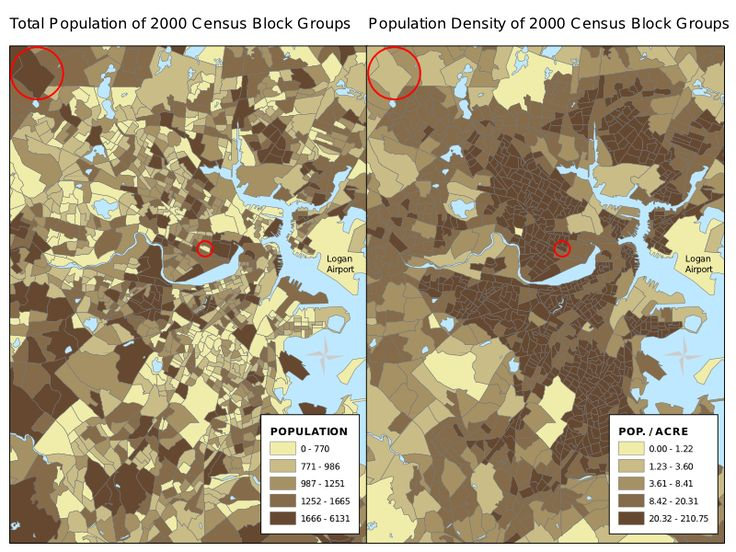
\includegraphics[width=.45\textwidth]{images/boston-density.jpg}
\caption{Mapa de densidade demográfica de bairros da cidade de Boston.}
\end{figure}


\end{frame}

%==================
\begin{frame}
\frametitle{Choropleth Map}
\justifying

\begin{columns}

\begin{column}{0.5\textwidth}


\end{column}

\begin{column}{0.5\textwidth}

\begin{figure}
\centering
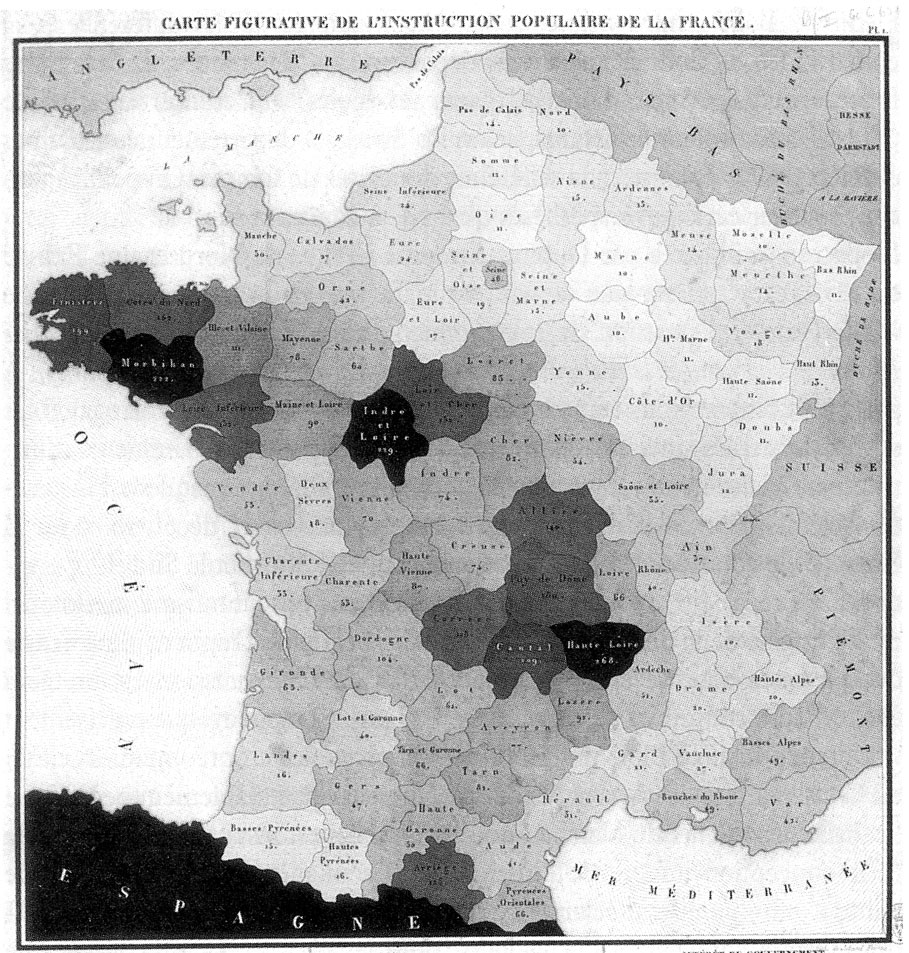
\includegraphics[width=.6\textwidth]{images/analfabetismo-franca.jpg}
\caption{Mapa da taxa de analfabetismo na França em 1826.}
\end{figure}


\end{column}
\end{columns}


\end{frame}

%==================
\section{Estudos de Caso}
\begin{frame}
\frametitle{Estudos de Caso}
\justifying


\end{frame}

\begin{frame}
\frametitle{Estudo de Caso I}
\justifying

\begin{figure}
\centering
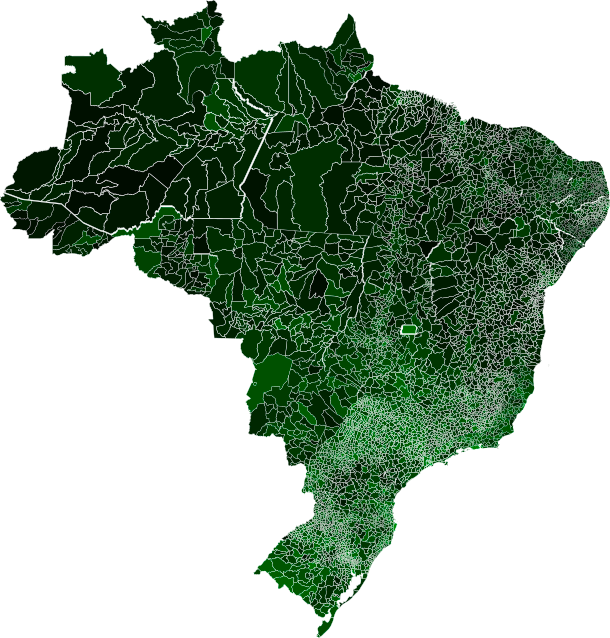
\includegraphics[width=0.33\textwidth]{images/educacao-1991.png}
\caption{IDHM Educação 1991.}
\end{figure}


\end{frame}

\begin{frame}
\frametitle{Estudo de Caso I}
\justifying

\begin{figure}
\centering
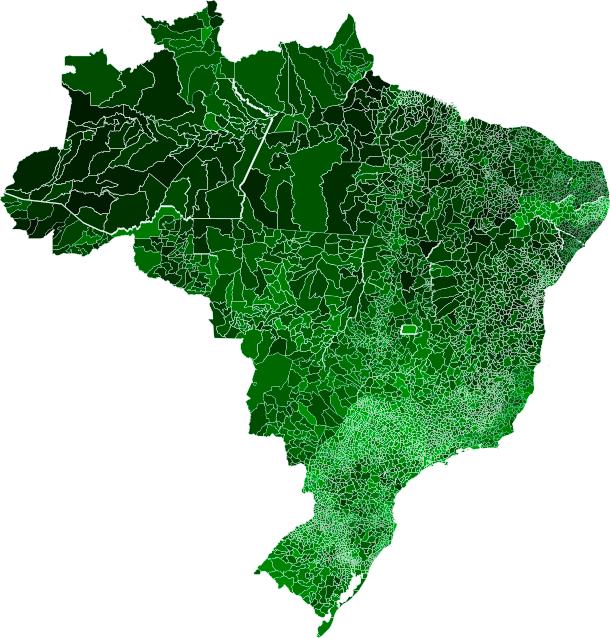
\includegraphics[width=0.33\textwidth]{images/educacao-2000.png}
\caption{IDHM Educação 2000.}
\end{figure}


\end{frame}

\begin{frame}
\frametitle{Estudo de Caso I}
\justifying

\begin{figure}
\centering
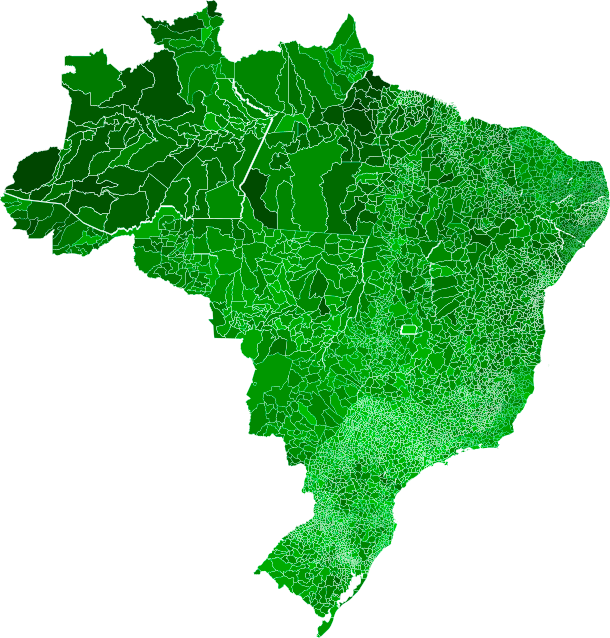
\includegraphics[width=0.33\textwidth]{images/educacao-2010.png}
\caption{IDHM Educação 2010.}
\end{figure}


\end{frame}

\begin{frame}
\frametitle{Estudo de Caso II}
\justifying

\begin{figure}
\centering
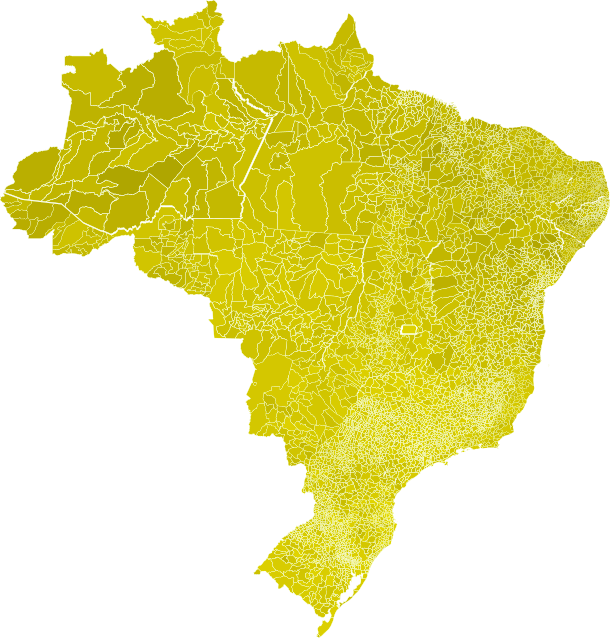
\includegraphics[width=0.33\textwidth]{images/longevidade.png}
\caption{IDHM Longevidade 2010.}
\end{figure}

\end{frame}

\begin{frame}
\frametitle{Estudo de Caso II}
\justifying

\begin{figure}
\centering
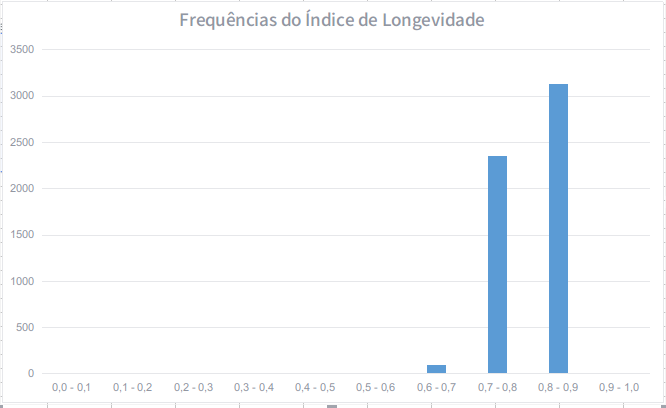
\includegraphics[width=0.33\textwidth]{images/frequencia.png}
\caption{Gráfico de distribuição de ocorrências.}
\end{figure}

\end{frame}

\begin{frame}
\frametitle{Estudo de Caso II}
\justifying

\begin{figure}
\centering
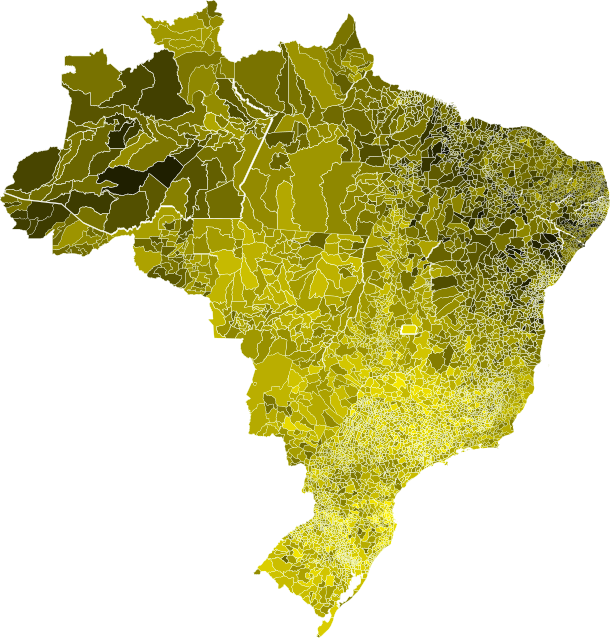
\includegraphics[width=0.33\textwidth]{images/longevidade-ampliado.png}
\caption{IDHM Longevidade 2010 Normalizado.}
\end{figure}

\end{frame}

\begin{frame}
\frametitle{Estudo de Caso III}
\justifying


\begin{figure}
\centering
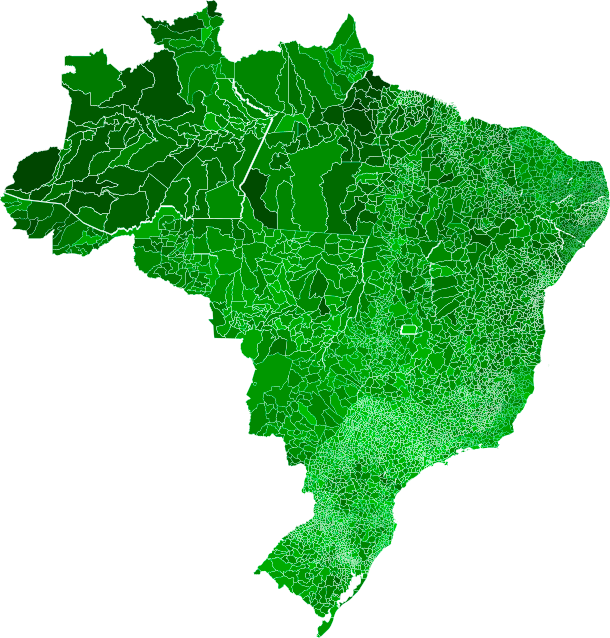
\includegraphics[width=0.33\textwidth]{images/educacao-2010.png}
\caption{IDHM Educação 2010.}
\end{figure}

\end{frame}

\begin{frame}
\frametitle{Estudo de Caso IV}
\justifying

\begin{figure}
\centering
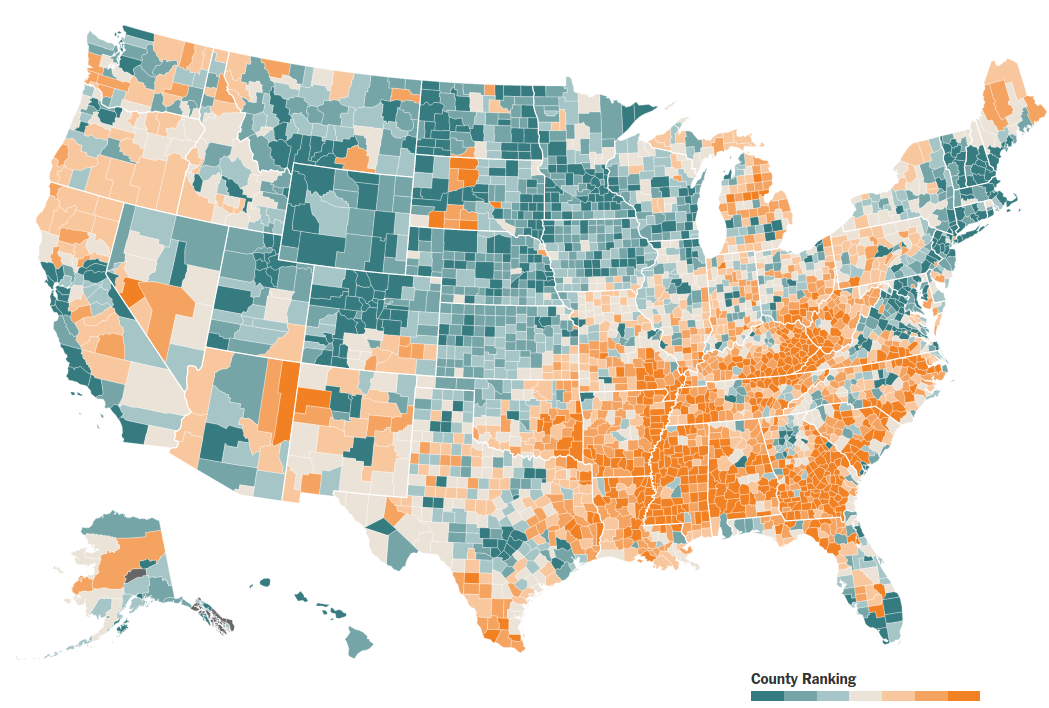
\includegraphics[width=0.6\textwidth]{images/usa.png}
\end{figure}


\end{frame}

\begin{frame}
\frametitle{Estudo de Caso IV}
\justifying

\begin{figure}
\centering
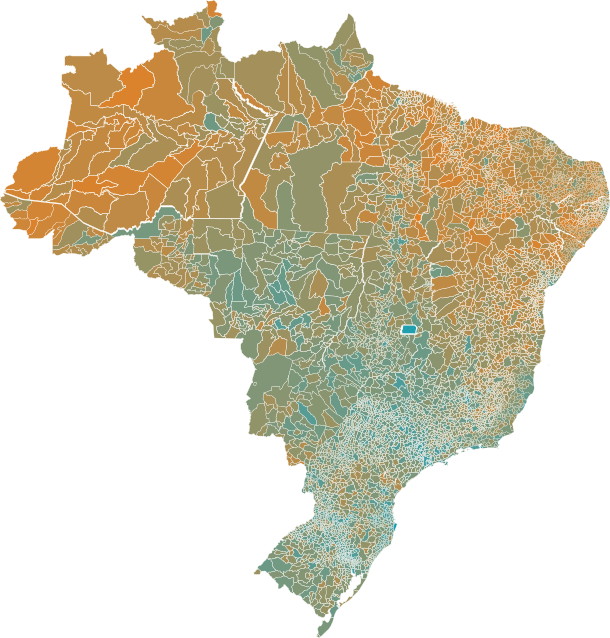
\includegraphics[width=0.4\textwidth]{images/qualidade-de-vida.png}
\end{figure}


\end{frame}

%================
\begin{frame}
\frametitle{Considerações Finais}
\justifying





\end{frame}


\end{document}

\end{document}
              
            